\documentclass[11pt,a4paper,oneside,ngerman]{scrartcl} %Deutschsprachiges Dokument mit der passenden Absatzkennzeichnung in der KOMA-Klasse article

\usepackage[T1]{fontenc} %Fontencoding T1 = skalierbare Vektorschrift
\usepackage[ngerman]{babel}
%\usepackage{xunicode}
\usepackage{polyglossia}
\setmainlanguage{german}
\usepackage{xltxtra}
\usepackage{graphicx} %Standard-Paket zum einbinden von Grafiken
\usepackage[bookmarks=true, bookmarksnumbered=false, bookmarksopen=false, colorlinks=true, linkcolor=black, citecolor=black, urlcolor=black]{hyperref}
\usepackage{amsmath}
\usepackage{cancel}
\usepackage{mathcomp}
\usepackage{lmodern,dsfont}
\usepackage{listings}
\usepackage{color}
\usepackage{soul}
\usepackage{setspace}
\usepackage{titlesec}
\usepackage{fancyhdr}
\usepackage{nameref}
\usepackage{microtype} %Verbesserte Trennregeln mithilfe von Mikrotypografie
\usepackage{csquotes} %Paket für kontextsensitive Zitate
\usepackage[output-decimal-marker={,},exponent-product=\cdot]{siunitx} %Paket für Einheiten mitsamt der deutschen Anpassungen
\usepackage[backend=biber, style=apa, language=ngerman, hyperref=true, url=true, backref=true, doi=false, isbn=false, eprint=false, sorting=anyt, maxalphanames=1, labelalpha, natbib=true]{biblatex} %Lade biblatex für die Erstellung der Bibliografie mit biber ohne Sortierung (Einträge werden nach Aufruf sortiert)
\usepackage{tabularx} %Paket für Tabellen mit variabler Breite um diese gleich der Seitenbreite zu setzen
\usepackage[section]{placeins} %Verhindert, dass Abbildungen außerhalbder aktuellen section gesetzt werden
\usepackage[noabbrev]{cleveref} %
\usepackage{epstopdf}
\usepackage{nicefrac}
\usepackage[draft, author={Max Mustermann}]{pdfcomment}
\usepackage{wasysym}
\usepackage{enumitem}

\def\fps@figure{htbp} %Standardpositionierung für Bilder und Tabellen auf htbp anstatt tbp
\def\fps@table{htbp} %Standardpositionierung für Tabellen auf htbp anstatt tbp
\setkeys{Gin}{width=\linewidth,height=\textheight,keepaspectratio} %Bildskalierung auf Seitenbreite
%Bilder zentriert einfügen
\makeatletter
\g@addto@macro\@floatboxreset\centering
\makeatother

%Trennung durch Komma bei mehrfachem \footcite
\usepackage{fnpct}
\AdaptNoteOpt\footcite\multfootcite

\addbibresource{library/literature.bib} %Einbinden der Bibliotheksdatenbank
\DeclareLanguageMapping{ngerman}{ngerman-apa}
%Übersetzungen für Bibliographie
\DefineBibliographyStrings{ngerman}{%
	andothers ={et\addabbrvspace al\adddot}, %et al.
	andmore   ={et\addabbrvspace al\adddot}, %et al.
	nodate    ={n\adddot d\adddot}, %n.d.
}
\addto\extrasngerman{%
	\def\subsectionautorefname{Abschnitt}% Setze den Autorefname von subsection von Unterabschnitt auf Abschnitt
}

% Hurenkinder und Schusterjungen
\clubpenalty10000
\widowpenalty10000
\displaywidowpenalty=10000

% page borders
\usepackage[a4paper,left=3.5cm,right=2.5cm,top=2.5cm,bottom=2.5cm]{geometry}

\newcommand{\getAuthor}{unbekannter Author}
\newcommand{\getTitle}{kein Titel}
\newcommand{\getSemester}{SS 12}
\newcommand{\getErstgutachter}{Kein Dozent}
\newcommand{\getZweitgutachter}{Kein Dozent}
\newcommand{\getDate}{\today}
\newcommand{\getStudID}{}
\newcommand{\getAddress}{}
\newcommand{\getDateHandedIn}{}
\renewcommand{\author}[1]{\renewcommand{\getAuthor}{#1\\}}
\renewcommand{\title}[1]{\renewcommand{\getTitle}{#1}}
\newcommand{\semester}[1]{\renewcommand{\getSemester}{#1}}
\newcommand{\erstgutachter}[1]{\renewcommand{\getErstgutachter}{#1\\}}
\newcommand{\zweitgutachter}[1]{\renewcommand{\getZweitgutachter}{#1\\}}
\newcommand{\studid}[1]{\renewcommand{\getStudID}{#1\\}}
\newcommand{\address}[2]{\renewcommand{\getAddress}{#1, #2\\}}
\newcommand{\dateHandedIn}[1]{\renewcommand{\getDateHandedIn}{#1}}
\newcommand{\writemeta}{
	\hypersetup{pdfinfo={
		Title={\getTitle},
		Author={\getAuthor}
	}}
}

\renewcommand*{\sectionmark}[1]{\markright{#1}}
\renewcommand{\abstract}{\noindent\begin{large}\textbf{Abstract}\end{large}\\\vspace*{10pt}\\}

\newcommand{\N}{\mathds{N}}

\newcommand{\img}[2]{
	\includegraphics[width=#2]{images/#1}
}

\renewcommand{\maketitle}{
\setstretch{1.0}
	
\vspace*{-30pt}
\hfill
\includegraphics[width=0.64\textwidth]{images/logo_uni}
\vspace*{20pt}
	
\vspace*{120pt}
	
\begin{center}
	\begin{huge}
		\sffamily\getTitle \\
	\end{huge}
	\vspace*{13pt}
	Masterarbeit im Fach Medieninformatik am \\
	Institut für Medien, Sprache und Kultur (I:IMSK)
\end{center}
	
\vfill

\par
\begingroup
\leftskip=4.9cm
\noindent
Vorgelegt von: \noindent\getAuthor
Adresse: \getAddress
Matrikelnummer: \getStudID
Erstgutachter: Prof. Dr. Erstgutachter\\
Zweitgutachter: Prof. Dr. Zweitgutachter\\
Laufendes Semester: \getSemester\\
Abgegeben am \getDateHandedIn
\par
\endgroup

}

% Code
\definecolor{maroon}{rgb}{0.5,0,0}
\definecolor{darkgreen}{rgb}{0,0.5,0}
\definecolor{gray}{rgb}{0.5,0.5,0.5}


\lstdefinelanguage{XML}
{
	basicstyle=\ttfamily\footnotesize,
	tabsize=2,
	frame=single,
	xleftmargin=15pt,
	framexleftmargin=10pt,
	numbers=left,
	numberstyle=\tiny,
	numbersep=5pt,
	breaklines=true,
	morestring=[s]{"}{"},
	morecomment=[s]{?}{?},
	morecomment=[s]{!--}{--},
	commentstyle=\color{darkgreen},
	moredelim=[s][\color{black}]{>}{<},
	moredelim=[s][\color{red}]{\ }{=},
	stringstyle=\color{blue},
	identifierstyle=\color{maroon}
}
\lstdefinelanguage{JSON}
{
	basicstyle=\ttfamily\footnotesize,
	numbers=left,
	numberstyle=\tiny,
	stepnumber=1,
	numbersep=5pt,
	showstringspaces=false,
	breaklines=true,
	frame=single,
	backgroundcolor=\color{white},
	morecomment=[s]{/*}{*/},
	commentstyle=\color{gray},
	tabsize=2,
	literate=
	 {:}{{{\color{maroon}{:}}}}{1}
	 {,}{{{\color{maroon}{,}}}}{1}
	 {\{}{{{\color{blue}{\{}}}}{1}
	 {\}}{{{\color{blue}{\}}}}}{1}
	 {[}{{{\color{blue}{[}}}}{1}
	 {]}{{{\color{blue}{]}}}}{1}	
}

% Schriftarten
\renewcommand{\familydefault}{\rmdefault}
\setromanfont{Palatino Linotype}
\setmonofont[Scale=1.0,BoldFont={* Medium}]{Source Code Pro}
\setsansfont[BoldFont={* Medium}]{Frutiger Next Pro}
%\setmainfont[BoldFont={* Medium}]{Frutiger Next Pro}

\titleformat*{\section}{\Large\bfseries\sffamily}
\titleformat*{\subsection}{\large\bfseries\sffamily}
\titleformat*{\subsubsection}{\itshape\bfseries\sffamily}

% Keep image inside subsection
\makeatletter
\AtBeginDocument{%
	\expandafter\renewcommand\expandafter\subsection\expandafter{%
		\expandafter\@fb@secFB\subsection
	}%
}
\makeatother

% Keep image inside subsubsection
\makeatletter
\AtBeginDocument{%
	\expandafter\renewcommand\expandafter\subsubsection\expandafter{%
		\expandafter\@fb@secFB\subsubsection
	}%
}
\makeatother

\title{Titel der Arbeit}
\author{Max Mustermann}
\semester{SS 2016}
\studid{1234567}
\address{Musterstraße 1}{12345 Musterhausen}
\dateHandedIn{31.07.2016}
\writemeta

\begin{document}

\maketitle
\thispagestyle{empty} % no page numbering on first page
\newpage

%Inhaltsverzeichnis----------------------------------------------------------------------------
\thispagestyle{empty} % no page numbering on table of contents page
\tableofcontents
\clearpage
%Ende Inhaltsverzeichnis-----------------------------------------------------------------------

%Abbildungsverzeichnis-------------------------------------------------------------------------
\thispagestyle{empty} % no page numbering on list of figures page
\listoffigures
\clearpage
%Ende Abbildungsverzeichnis--------------------------------------------------------------------

\pagestyle{fancy}
\fancyhead[R]{\sffamily\thepage}
\fancyhead[L]{\sffamily\nouppercase{\leftmark}}
\fancyfoot[C]{\empty}
\setstretch{1.5}

%Kapitelabschnitte-----------------------------------------------------------------------------
\section{Über dieses Dokument}
Dieses Dokument soll Ihnen den Einstieg beim Verfassen einer Studienarbeit erleichtern. Die Vorgaben sind als Empfehlungen zu verstehen, können aber bei Bedarf in Absprache mit den Dozenten angepasst und erweitert werden. Hier steht ein Beispielabschnitt. Die Schriftart ist Frutiger Next Pro, die 
Schriftgröße 11pt. Ein Verweis auf eine Abbildung (vgl. \cref{fig:norman2002}) wird in diesem Satz verdeutlicht. Alternativ eignen sich auch Serifenschriftarten wie Garamond, Times New Roman oder Frutiger Serif Pro. Querverweise (vgl. \cref{sec:ein-unterabschnitt}) werden in diesem Satz  gezeigt. Der erste Absatz jedes Abschnitts und Absätze nach Abbildungen werden nicht eingerückt (Formatvorlage ist Standard). Ein weiterer Absatz wird durch Drücken der Return-Taste erzeugt und automatisch eingerückt. Absätze werden also nicht durch Leerzeilen, sondern durch Einrücken des Folgeabsatzes getrennt. Die Folgeabsätze erhalten automatisch die Formatvorlage Folgeabsatz.

In dieser Vorlage können auch Codeschnipsel eingesetzt und referenziert werden (vgl. Algorithmus:).

In der Kopfzeile erscheint immer der Text der aktuellen Überschrift, die mit der Formatvorlage \enquote{Überschrift 1} formatiert wird. Somit wird dem Leser die Orientierung in der Arbeit erleichtert.
\begin{figure}[htbp]
	\centering
	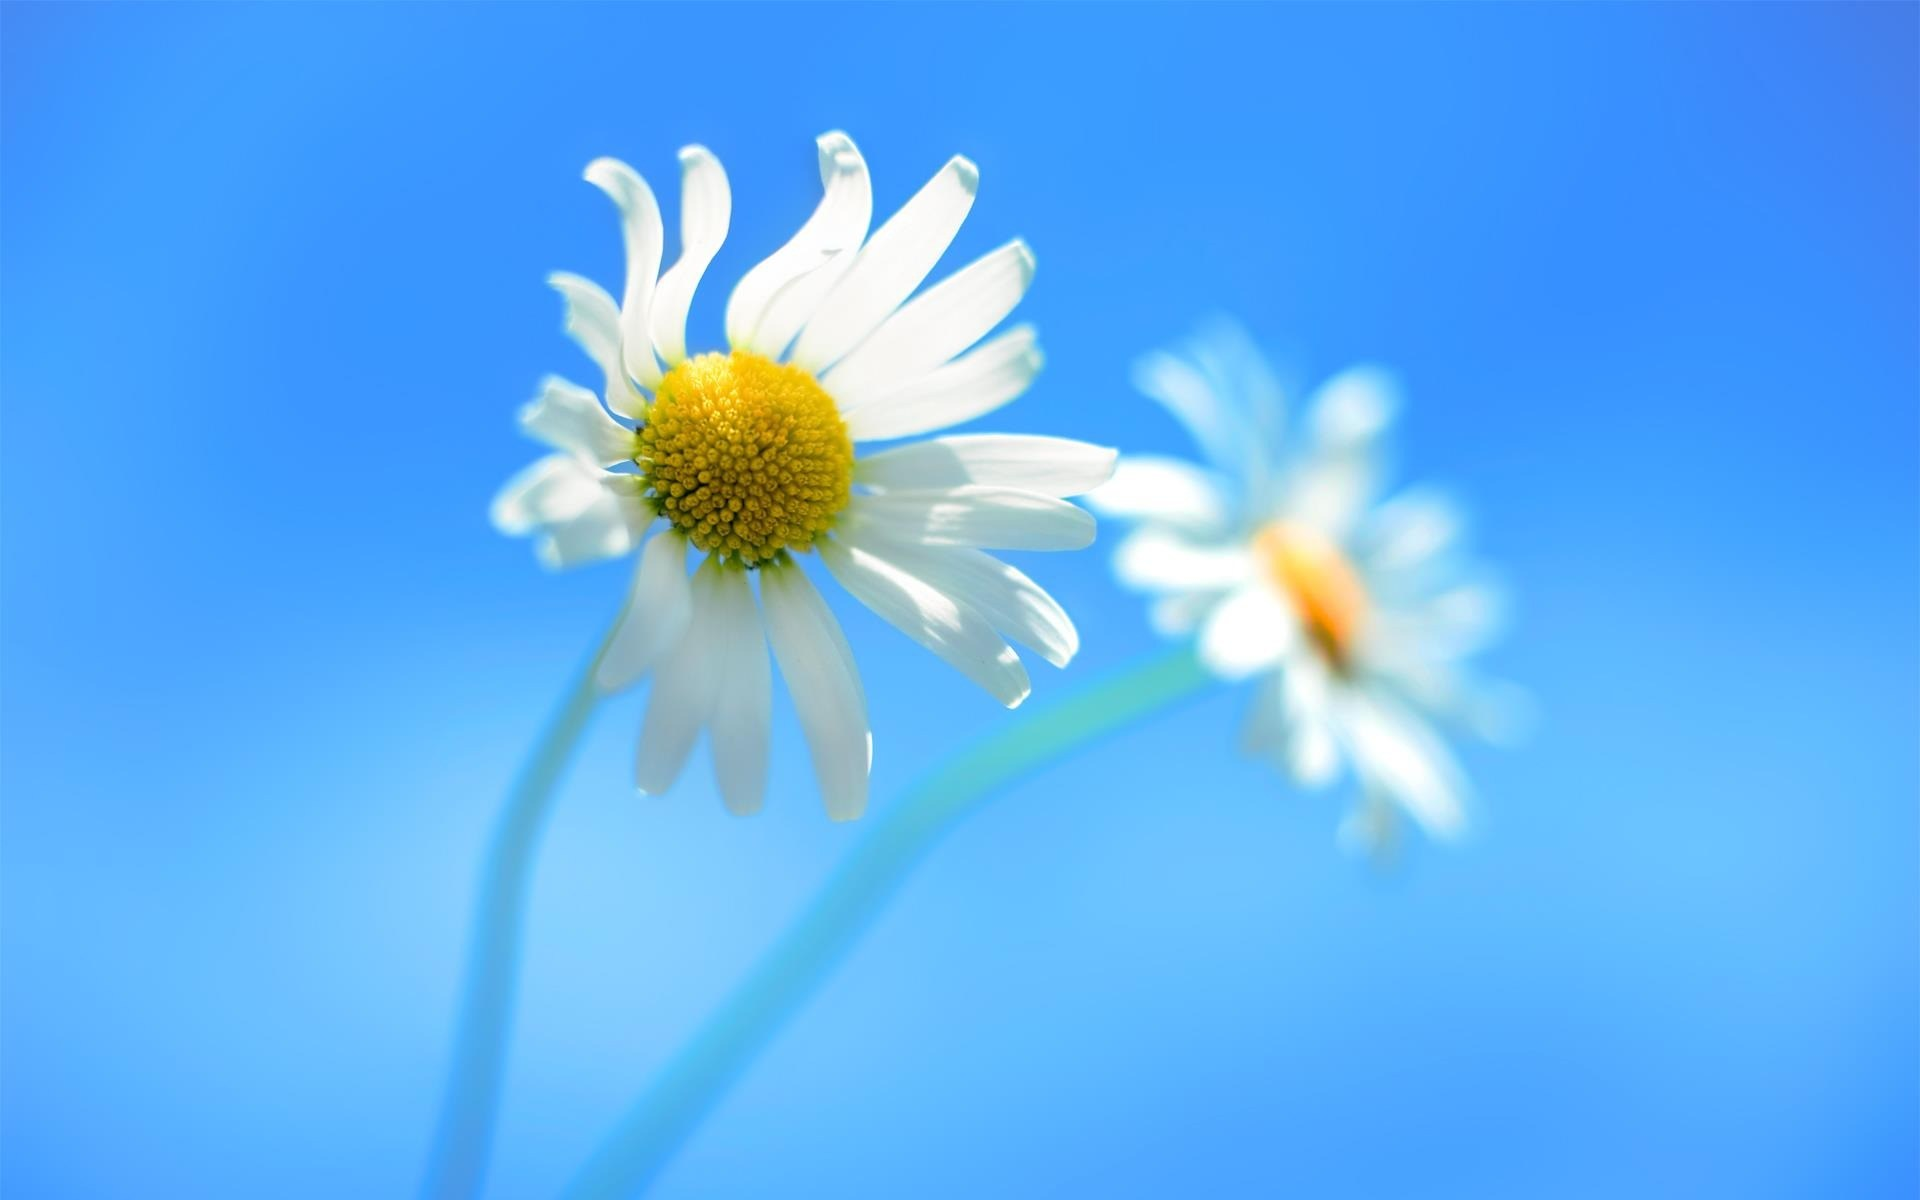
\includegraphics{images/demo}
	\caption{Blümchen \autocite{Norman:2002}}
	\label{fig:norman2002}
\end{figure}

\subsection{Ein Unterabschnitt}\label{sec:ein-unterabschnitt}
Ein Beispiel für einen Codeschnipsel in JSON:
\lstset{
	language=JSON,
}
\lstinputlisting{code/format.json}
\section{Ein weiterer Abschnitt}\label{sec:ein-weiterer-abschnitt}
Lorem ipsum dolor sit amet, consetetur sadipscing elitr, sed diam nonumy eirmod tempor invidunt ut labore et dolore magna aliquyam erat, sed diam voluptua. At vero eos et accusam et justo duo dolores et ea rebum. Stet clita kasd gubergren, no sea takimata sanctus est Lorem ipsum dolor sit amet. Lorem ipsum dolor sit amet, consetetur sadipscing elitr, sed diam nonumy eirmod tempor invidunt ut labore et dolore magna aliquyam erat, sed diam voluptua. At vero eos et accusam et justo duo dolores et ea rebum. Stet clita kasd gubergren, no sea takimata sanctus est Lorem ipsum dolor sit amet.

Mit einer mathematischen Berechnung:
\begin{align*}
x &= (a_{2} + b_{2} * k) - (a_{1} + b_{1} * k) \\
((1;4),(4;4)) &= (4 + 4 * 12) - (1 + 4 * 12) \\
((1;4),(4;4)) &= 5
\end{align*}

\subsection{Ein weiterer Unterabschnitt}
Hier ein Codebeispiel in XML:
\lstset{
	language=XML,
}
\lstinputlisting{code/duration.xml}

\clearpage
%Ende Kapitelabschnitte------------------------------------------------------------------------

%Literaturverzeichnis--------------------------------------------------------------------------
\printbibliography
\clearpage
%Ende Literaturverzeichnis---------------------------------------------------------------------

%Plagiatserklärung-----------------------------------------------------------------------------
\newpage
\thispagestyle{empty} % no page numbering on table of contents page
\section*{Erklärung zur Urheberschaft}
Ich habe die Arbeit selbständig verfasst, keine anderen als die angegebenen Quellen und Hilfsmittel benutzt, sowie alle Zitate und Übernahmen von fremden Aussagen kenntlich gemacht.\\
Die Arbeit wurde bisher keiner anderen Prüfungsbehörde vorgelegt.\\
Die vorgelegten Druckexemplare und die vorgelegte digitale Version sind identisch.\\


\vspace{55pt}
\null\parbox{5.5cm}{\hrulefill\\\raggedright Ort, Datum}
\null\hfill\parbox{5.5cm}{\hrulefill\\\raggedleft Unterschrift}

\clearpage

\section*{Erklärung zur Lizenzierung und Publikation dieser Arbeit}
Hiermit gestatte ich die Verwendung der \textbf{schriftlichen Ausarbeitung} zeitlich unbegrenzt und nicht-exklusiv unter folgenden Bedingungen:

\begin{enumerate}[noitemsep]
	\item[\Square] Nur zur Bewertung dieser Arbeit
	\item[\Square] Nur innerhalb des Lehrstuhls im Rahmen von Forschung und Lehre
	\item[\XBox] Unter einer Creative-Commons-Lizenz mit den folgenden Einschränkungen:
	\begin{enumerate}[noitemsep]
		\item[\XBox] BY - Namensnennung des Autors
		\item[\Square] NC - Nichtkommerziell
		\item[\Square] SA - Share-Alike, d.h. alle Änderungen müssen unter die gleiche Lizenz gestellt werden.
	\end{enumerate}
\end{enumerate}

{
	\noindent\footnotesize (An Zitaten und Abbildungen aus fremden Quellen werden keine weiteren Rechte eingeräumt.)\\
}

\noindent Außerdem gestatte ich die Verwendung des im Rahmen dieser Arbeit erstellten \textbf{Quellcodes} unter folgender Lizenz:
\begin{enumerate}[noitemsep]
	\item[\Square] Nur zur Bewertung dieser Arbeit
	\item[\Square] Nur innerhalb des Lehrstuhls im Rahmen von Forschung und Lehre
	\item[\Square] Unter der CC-0-Lizenz (= beliebige Nutzung)
	\item[\XBox] Unter der MIT-Lizenz (= Namensnennung)
	\item[\Square] Unter der GPLv3-Lizenz (oder neuere Versionen)
\end{enumerate}

{
	\noindent\footnotesize (An explizit mit einer anderen Lizenz gekennzeichneten Bibliotheken und Daten werden keine weiteren Rechte eingeräumt.)\\
}

\noindent Ich willige ein, dass der Lehrstuhl für Medieninformatik diese Arbeit - falls sie besonders gut ausfällt - auf dem Publikationsserver der Universität Regensburg veröffentlichen lässt.

\noindent Ich übertrage deshalb der Universität Regensburg das Recht, die Arbeit elektronisch zu speichern und in Datennetzen öffentlich zugänglich zu machen. Ich übertrage der Universität Regensburg ferner das Recht zur Konvertierung zum Zwecke der Langzeitarchivierung unter Beachtung der Bewahrung des Inhalts (die Originalarchivierung bleibt erhalten). Ich erkläre außerdem, dass von mir die urheber- und lizenzrechtliche Seite (Copyright) geklärt wurde und Rechte Dritter der Publikation nicht entgegenstehen.
\begin{enumerate}[noitemsep]
	\item[\XBox] Ja, für die komplette Arbeit inklusive Anhang
	\item[\Square] Ja, für eine um vertrauliche Informationen gekürzte Variante (auf dem Datenträger beigefügt)
	\item[\Square] Nein
\end{enumerate}
\begin{enumerate}[noitemsep]
	\item[\Square] Sperrvermerk bis (Datum):
\end{enumerate}

\vspace{55pt}
\null\parbox{5.5cm}{\hrulefill\\\raggedright Ort, Datum}
\null\hfill\parbox{5.5cm}{\hrulefill\\\raggedleft Unterschrift}
\clearpage
%Ende Plagiatserklärung------------------------------------------------------------------------

\end{document}
